\subsection{24. Алгоритм Эрли синтаксического разбора для КС-грамматик: обоснование сложности. Примеры случаев, где Эрли ведёт себя квадратично. Как реализовать алгоритм Эрли, чтобы он был эффективным}

\textbf{Эффективное хранение ситуаций и правил}

Требуется эффективным образом хранить ситуации типа $\{A \rightarrow \alpha \cdot X \beta, i\} \in D_j$. Множества $D_j$ можно хранить в массиве $D[j][X]$, где $D[j][X] = \{(A_1 \rightarrow \alpha_1 \cdot X \beta_1, i_1), (A_2 \rightarrow \alpha_2 \cdot X \beta_2, i_2), \dots \}$. Возможны три случая, связанные с символом $X$:

\begin{enumerate}
    \item $X = a$, $a \in \Sigma$
    
    \item $X = B$, $B \in N$
    
    \item $X = \$$, $\$$ — конец слова
\end{enumerate}

Правила будем хранить в массиве $G[A]$, где в $G[A]$ будут храниться все правила начинающиеся с $A$, то есть правила вида $A \rightarrow \beta$.

\textbf{Об операциях}

Пусть $w$ — слово.
\begin{enumerate}
\item Scan. $\forall j < |w|:$ $w[j] = a$. Тогда нужно рассмотреть все элементы $D[j][a]$ и расположить их в $D[j + 1]$ в соответствии с символом, следующим за $a$. Асимптотика этой операции соответствует $\mathcal{O} (D[j][a])$, то есть она растёт в соответствии с количеством элементов, находящихся в $D[j][a]$.

\item Predict. $\forall j, B:$ Пусть ситуация имеет вид $(A \rightarrow \alpha \cdot B \beta, i) \in D_j$. Она лежит в $D[j][B]$. Нужно рассмотреть все правила вида $B \rightarrow \gamma \in P$, они лежат в $G[B]$. Асимптотика этой операции $O(D[j][B] \cdot G[B])$.

\item Complete. $\forall j, B:$ Пусть ситуация имеет вид $(B \rightarrow \gamma \cdot, i) \in D_j$, она лежит в $D[j][\$]$. Нужно рассмотреть все ситуации вида $(A \rightarrow \alpha \cdot B \beta, k) \in D_i$, они лежат в $D[i][B]$. Асимптотика этой операции $O(\sum_{i \leq j} G[B] \cdot D[i][B])$.
\end{enumerate}

\textbf{Оценки}

Оценим, как растёт величина $|D_j|$. $D_j = \{(A_1 \rightarrow \alpha_1 . \beta_1, i_1), (A_2 \rightarrow \alpha_2 . \beta_2, i_2), \dots \}$. Пусть $|G|$ — сумма всех длин правых частей правил. Значение $i$ может быть от $0$ до $j$, а точка может быть расположена в $\mathcal{O} (|G|)$ мест, поэтому $\mathcal{O} (|D_j|) = (j + 1)|G|$. 

Асимптотика операции Scan соответствует $\mathcal{O} (|D_j|) = \mathcal{O} (|w| \cdot |G|)$.\\
Асимптотика всех операций Scan $\mathcal{O} (|D_j| \cdot |w|) = \mathcal{O} (|w|^2 \cdot |G|)$.

Для оценки асимптотики операции Predict рассмотрим множества вида:

\begin{center}
    $(A \rightarrow \alpha \cdot B \beta, i) \in D_j$
    
    $(B \rightarrow \cdot \gamma, j) \in D_j$
\end{center}

Так как операция Predict сводится к перебору по $i$, точке и правилам левая часть которых $B$, то асимптотика операции соответствует $\mathcal{O} (D[j][B] \cdot G[B]) = \mathcal{O} (|w| \cdot |G| \cdot G[B])$.

Асимптотика всех операций Predict $O( \sum_{j, B} D[j][B] \cdot G[B] ) = O( |P| \cdot |G| \cdot |w|^2 )$, где $P$ - множество всех правил. 

Рассмотрим теперь операцию Complete. Ситуации из $D[j][\$]$ указывают на номер множества $i$ и нетерминальный символ $B$, который соответствует левой части правила из ситуации. Поэтому для каждой ситуации из $D[j][\$]$ будут рассмотрены все ситуации из $D[i][B]$. Поэтому асимптотика всех операций Complete равна $O(\sum_{j, i \leq j, B} G[B] \cdot D[i][B]) = O(\sum_{j, i \leq j, B} G[B] \cdot D_i) = O(\sum_{j, i \leq j} |P| \cdot D_i) = \mathcal{O} (|P| \cdot |w|^2 \cdot |w| \cdot |G|) = \mathcal{O} ({|w|}^3 {|G|}^2)$.

Так как итераций $\mathcal{O} (|w|)$, то итоговая сложность алгоритма составляет $\mathcal{O} ({|w|}^3{|G|}^2)$. Однако данную оценку можно сильно улучшить, если грамматически удастся доказать (на лекции не стали доказывать), что количество появлений каждого правила ограничена сверху некоторой константой $C$, то асимптотика уже будет равна $\mathcal{O} ({|w|}^2 \cdot C)$. Считаем $|P|, |G|, C$, константами, потому что "вся эта история происходит на стадии компиляции". (в алгоритме мы работаем с одним набором правил, видимо поэтому эти величины можно считать константой)

Есть теорема, что если грамматика однозначна, то алгоритм Эрли для неё стоит квадрат.
Идея доказательства в том, что если грамматика однозначна, то в complete в $(A \rightarrow \alpha \cdot B \beta, k) \in D_i, (B \rightarrow \cdot \gamma, i) \in D_j$ не нужно будет перебирать $i$. Оно будет подбираться однозначно.

Алгоритм за куб.

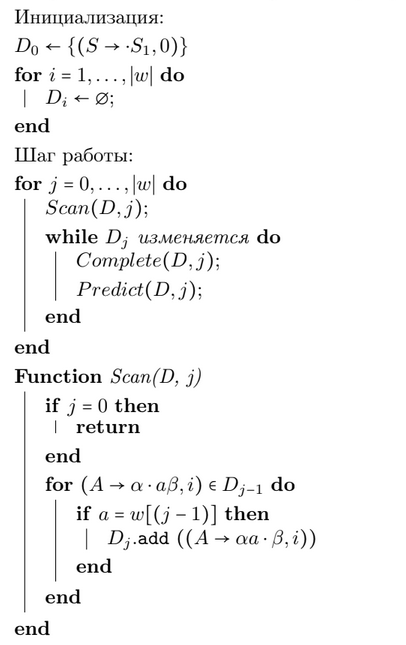
\includegraphics[width=0.45\linewidth]{24_1.png}

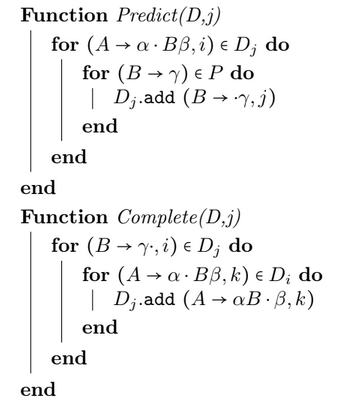
\includegraphics[width=0.4\linewidth]{24_2.png}

Эффективный алгоритм и примеры случаев, где Эрли ведёт себя квадратично: (из neerc.ifmo)

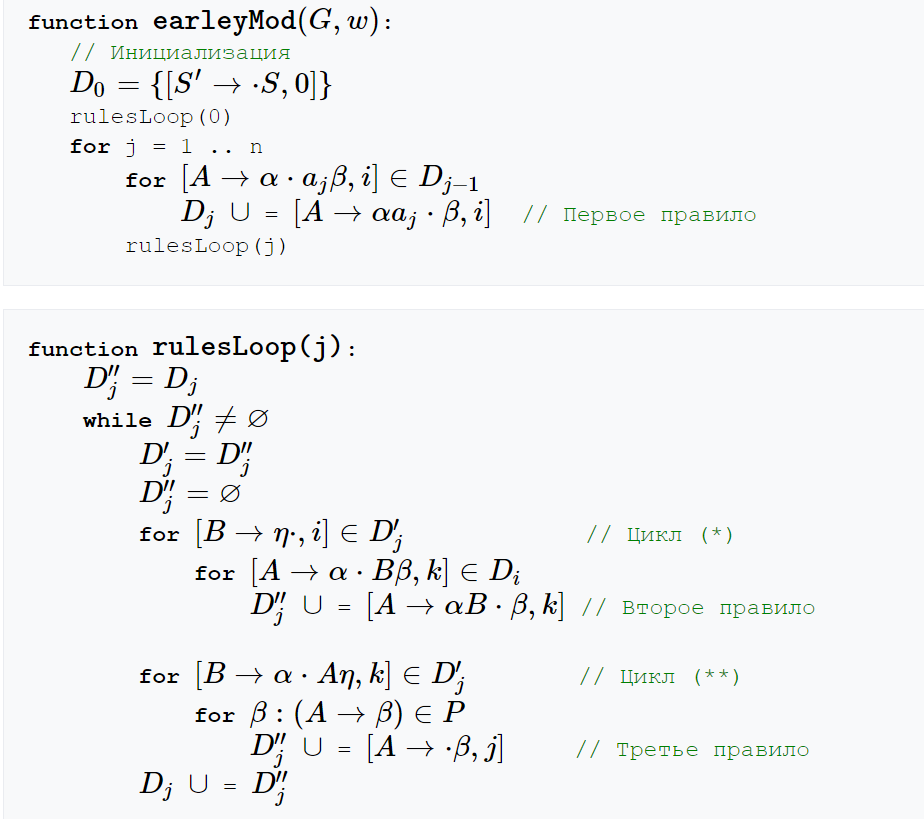
\includegraphics[width=0.8\linewidth]{24_3.png}

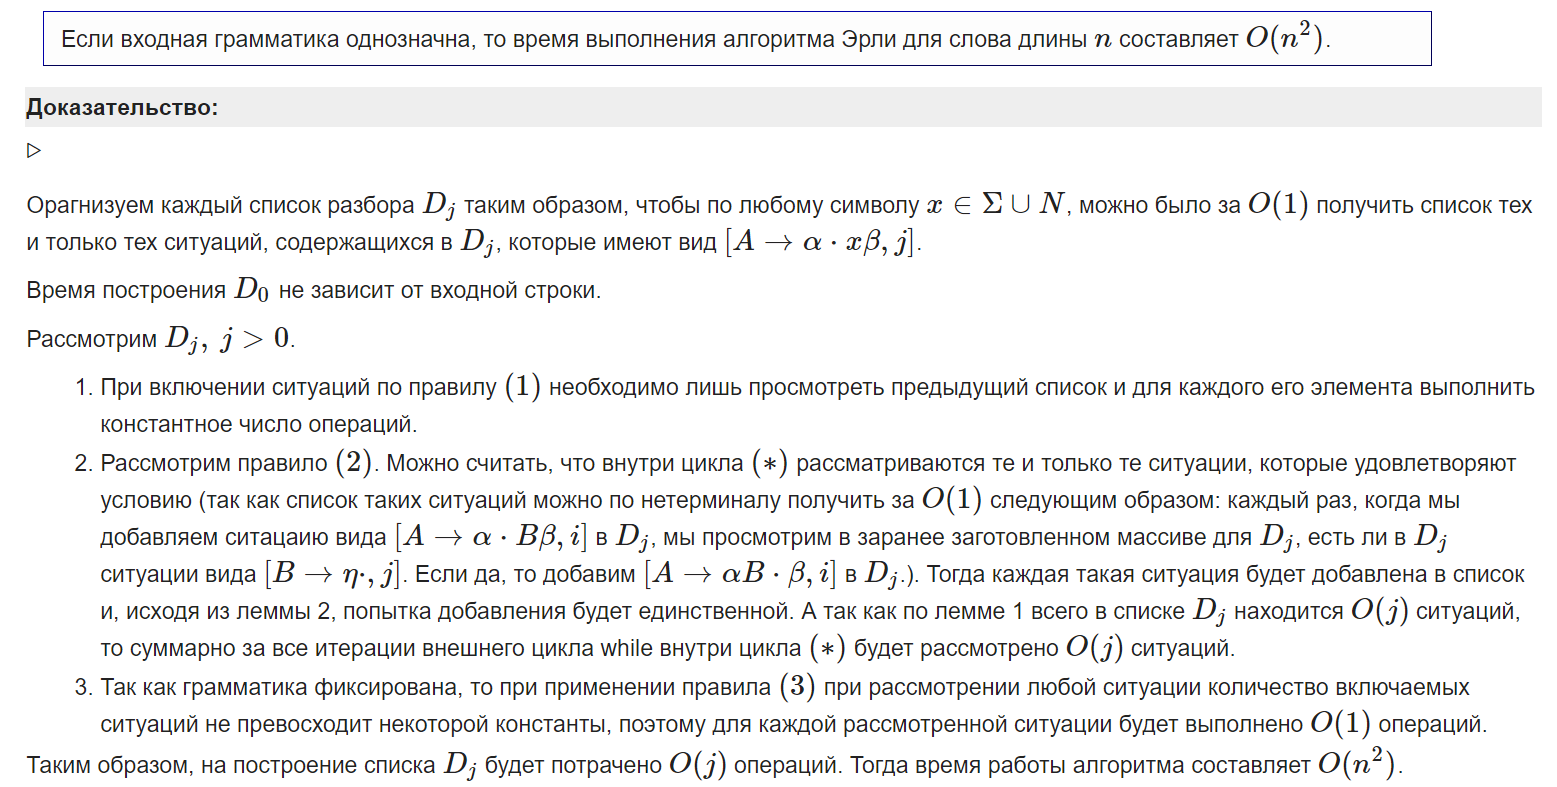
\includegraphics[width=1\linewidth]{24_4.png}